\chapter{Calculer un $Q$ pour un $T_\text{retour}$ donné -- \textit{Séries annuelles}}

Nous avons les données suivantes :
\begin{table}[H]
    \centering
    \begin{tabular}{|c||c|c|c|c|c|c|c|c|c|c|c|c|}
        \hline
        \textbf{Année} & \textbf{Jan} & \textbf{Fev} & \textbf{Mar} & \textbf{Avr} & \textbf{Mai} & \textbf{Juin} & \textbf{Jui} & \textbf{Aoû} & \textbf{Sep} & \textbf{Oct} & \textbf{Nov} & \textbf{Dec} \\
        \hline \hline
        \textbf{1965}  & 11 & \cellcolor{green}10 & 14 & 15 & 160 & 205 & 205 & \cellcolor{red}350 & 145 &  84 &  21 & 18 \\
        \hline
        \textbf{1966}  & \cellcolor{green}17 & 19 & 17 & 47 & 105 & \cellcolor{red}175 & 155 & 150 &  97 & 125 &  25 & 20 \\
        \hline
        \textbf{\dots} &    &    &    &    &     &     &     &     &       &     &     &      \\
        \hline
        \textbf{1992}  & 14 & \cellcolor{green}13 & 17 & 62 & 110 & \cellcolor{red}290 & 225 & 215 & 175 &  75 &  46 & 38 \\
        \hline
        \textbf{1993}  & 28 & 42 & 38 & 49 & 125 & 200 & 180 & 150 & \cellcolor{red}460 & 170 &  37 & \cellcolor{green}27 \\
        \hline
    \end{tabular}
    \caption{Tableau avec les débits maximums pour chaque mois entre les années 1965 et 1993}
    \label{tab:seriesAnnuellesMaximum}
\end{table}


\section{Contrôler la stationnarité}
Le contrôle de la stationnarité se fait en créant le graphique des débits maximales par années (cf. Figure \ref{graph:stationnarite})
\begin{figure}[H]
    \centering
    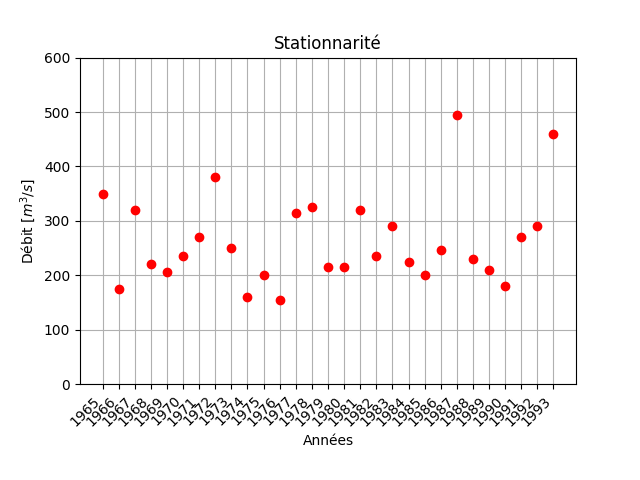
\includegraphics[width=12cm]{stationnarite.png}
    \caption{Stationnarité (étude entre 1965 et 1993)}
    \label{graph:stationnarite}
\end{figure}


\section{Contrôler l'homogénéité -- \textit{Optionnel}}
Afin de contrôler l'homogénéité des débits, il faut tracer un graphique avec les débits maximums mensuels et pour toutes les années (cf. Figure \ref{graph:homogeneite}).
\begin{figure}[H]
    \centering
    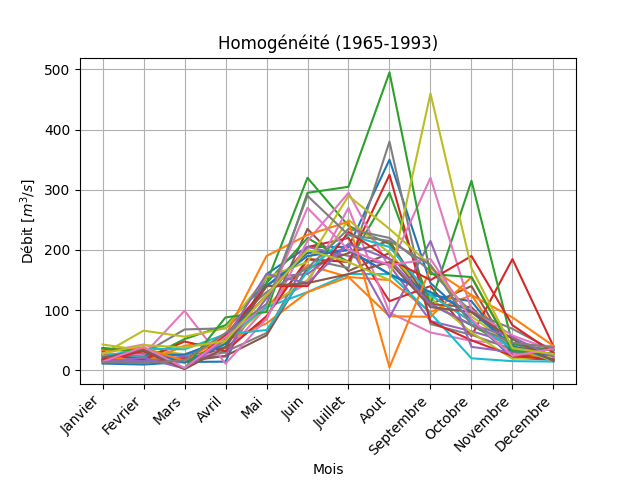
\includegraphics[width=12cm]{homogeneite.png}
    \caption{Homogénéité (étude entre 1965 et 1993)}
    \label{graph:homogeneite}
\end{figure}